\section{Hệ Thống Đề Xuất}\label{sec2a}

Phần này trình bày hệ thống mạng điều khiển đèn giao thông thông minh toàn diện tích hợp 
Học Sâu Tăng Cường (DRL) với các công nghệ thị giác máy tính để quản lý giao thông thích ứng. 
Hệ thống đề xuất sử dụng kiến trúc phân cấp kết hợp khả năng ra quyết định cục bộ và toàn cục 
để đạt được sự phối hợp giao thông tối ưu trên nhiều nút giao thông.

\subsection{Tổng Quan Kiến Trúc Hệ Thống}\label{subsec2a-1}

Hệ thống điều khiển đèn giao thông thông minh đề xuất sử dụng kiến trúc phân cấp ba lớp được 
thiết kế để cân bằng khả năng phản ứng thời gian thực với tối ưu hóa toàn mạng. 
Hình~\ref{fig:system_overview} minh họa kiến trúc tổng thể của hệ thống.

\begin{figure}[!htb]
    \centering
    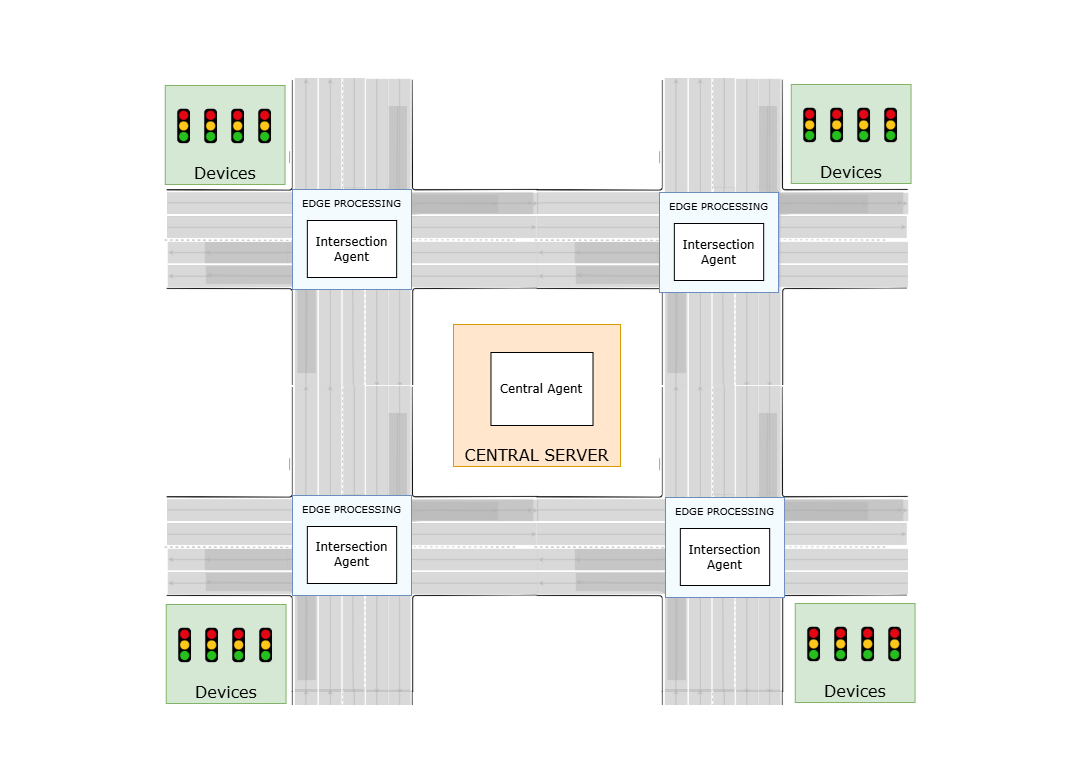
\includegraphics[width=0.8\textwidth]{figures/ch3_system_overview_architecture.png}
    \caption{Kiến trúc tổng thể hệ thống cho mạng điều khiển đèn giao thông thông minh}
    \label{fig:system_overview}
\end{figure}

Kiến trúc bao gồm ba lớp chính:

\textbf{Lớp Thiết Bị:} Camera giám sát được lắp đặt tại các nút giao thông thu thập luồng video 
thời gian thực về điều kiện giao thông. Những camera này được định vị chiến lược để cung cấp 
phạm phủ toàn diện cho tất cả các làn đường tiếp cận tại mỗi nút giao thông, đảm bảo khả năng 
hiển thị hoàn toàn về chuyển động xe và mô hình giao thông.

\textbf{Lớp Xử Lý Biên:} Các thiết bị tính toán cục bộ tại mỗi nút giao thông thực hiện phát hiện xe, 
theo dõi và điều khiển tín hiệu giao thông cục bộ theo thời gian thực. Cách tiếp cận phân tán này 
giảm thiểu độ trễ truyền thông và đảm bảo phản ứng ngay lập tức với điều kiện giao thông thay đổi. 
Mỗi nút giao thông hoạt động độc lập trong khi duy trì khả năng phối hợp với hệ thống trung tâm.

\textbf{Lớp Máy Chủ Trung Tâm:} Hệ thống phối hợp tập trung thu thập thông tin từ tất cả các tác nhân 
nút giao thông, đưa ra quyết định tối ưu hóa toàn cục và cung cấp giao diện quản lý thống nhất 
cho các nhà điều hành giao thông. Máy chủ trung tâm triển khai Tác nhân Đồng bộ phối hợp nhiều 
nút giao thông để tối ưu hóa luồng giao thông toàn mạng.

\subsection{Mô-đun Thị Giác Máy Tính}\label{subsec2a-2}

Mô-đun thị giác máy tính phục vụ như thành phần cảm biến của hệ thống, trích xuất thông tin 
giao thông toàn diện từ nguồn cấp camera sử dụng các thuật toán phát hiện và theo dõi đối tượng tiên tiến.

\subsubsection{Phát Hiện Xe với YOLO11}

Hệ thống sử dụng YOLO11s (You Only Look Once phiên bản 11 nhỏ), một mô hình được huấn luyện trước 
cung cấp sự cân bằng tối ưu giữa độ chính xác phát hiện và tốc độ xử lý cho các ứng dụng giao thông 
thời gian thực. YOLO11s đạt được 47.0 mAP$^{50-95}$ trên bộ dữ liệu COCO trong khi duy trì tốc độ 
xử lý hiệu quả phù hợp cho phân tích giao thông thời gian thực trên phần cứng hiện đại.

YOLO11s cung cấp một số ưu điểm chính cho các ứng dụng giao thông. Mô hình cung cấp hiệu suất cân bằng 
thông qua độ chính xác cao kết hợp với tốc độ suy luận nhanh phù hợp cho giám sát giao thông thời gian thực. 
Kiến trúc hiệu quả của nó có thiết kế backbone và neck được cải tiến với chỉ 9.4 triệu tham số, 
đảm bảo hiệu quả tính toán. Ngoài ra, khả năng được huấn luyện trước cho phép áp dụng trực tiếp 
vào các kịch bản giao thông mà không cần huấn luyện bổ sung, với hỗ trợ toàn diện cho các lớp xe 
bao gồm ô tô, xe máy, xe buýt và xe tải.

\subsubsection{Thuật Toán Theo Dõi Đối Tượng}

Để duy trì danh tính xe qua các khung hình video và trích xuất thông tin quỹ đạo, hệ thống triển khai 
hai thuật toán theo dõi bổ sung:

\textbf{SORT (Simple Online and Realtime Tracking):} Kết hợp bộ lọc Kalman với thuật toán Hungary để 
theo dõi đối tượng hiệu quả. Thuật toán thực hiện dự đoán vị trí sử dụng các mô hình chuyển động, 
gán đối tượng dựa trên khoảng cách IoU và cập nhật trạng thái với thông tin phát hiện mới.

\textbf{BotSORT:} Cải tiến SORT bằng cách tích hợp các tính năng dựa trên ngoại hình và các mô hình 
chuyển động được cải tiến, cung cấp độ chính xác theo dõi vượt trội trong các kịch bản phức tạp 
với sự che khuất thường xuyên và điều kiện giao thông dày đặc.

\subsection{Kiến Trúc Học Tăng Cường Phân Cấp}\label{subsec2a-3}

Hệ thống đề xuất sử dụng kiến trúc DRL phân cấp hai cấp giải quyết cả thách thức tối ưu hóa cục bộ 
và phối hợp toàn cục trong điều khiển giao thông đa nút giao thông.

\subsubsection{Cấp Cục Bộ: Các Tác Nhân DQN}

Mỗi nút giao thông được điều khiển bởi một tác nhân Deep Q-Network (DQN) chuyên dụng chịu trách nhiệm 
cho các quyết định tín hiệu giao thông cục bộ. Kiến trúc DQN có lớp đầu vào 80 chiều nắm bắt thông tin 
trạng thái giao thông toàn diện bằng cách chia mỗi hướng tiếp cận thành 8 nhóm làn đường (2 nhóm mỗi hướng: 
làn đi thẳng/rẽ phải và làn rẽ trái) với mỗi nhóm được phân đoạn thành 10 ô không gian, tạo ra vectơ 
trạng thái 8×10 = 80 phần tử. Mạng sử dụng bốn lớp ẩn kết nối đầy đủ với 400 nơ-ron mỗi lớp, 
sử dụng các hàm kích hoạt ReLU để biến đổi tính năng phi tuyến. Lớp đầu ra tạo ra các giá trị Q 
cho bốn pha giao thông có thể: xanh Bắc-Nam, xanh Đông-Tây, rẽ trái Bắc-Nam và rẽ trái Đông-Tây.

Không gian hành động được thiết kế để bao phủ các kịch bản điều khiển nút giao thông bốn hướng tiêu chuẩn, 
trong khi biểu diễn trạng thái nắm bắt cả động lực giao thông không gian và thời gian cần thiết 
cho việc ra quyết định thông minh.

\subsubsection{Cấp Toàn Cục: Tác Nhân SAC}

Tác nhân Đồng bộ sử dụng thuật toán Soft Actor-Critic (SAC) để phối hợp nhiều tác nhân DQN nút giao thông. 
SAC được chọn vì hiệu suất vượt trội trong không gian hành động liên tục và khả năng duy trì cân bằng 
khám phá-khai thác hiệu quả.

Tác nhân SAC quan sát thông tin tổng hợp từ tất cả các tác nhân DQN nút giao thông và đưa ra các quyết định 
phối hợp toàn diện. Những quyết định này bao gồm điều chỉnh thời lượng pha để phối hợp sóng giao thông, 
gán ưu tiên trong tình huống khẩn cấp, cân bằng tải trên mạng nút giao thông và tối ưu hóa thời gian 
đồng bộ để tăng cường luồng giao thông trên toàn mạng.

\subsection{Thiết Kế Hàm Phần Thưởng}\label{subsec2a-4}

Các hàm phần thưởng được thiết kế cẩn thận để tối ưu hóa nhiều mục tiêu giao thông đồng thời 
trong khi đảm bảo tính ổn định và hội tụ của hệ thống.

Đối với các tác nhân DQN nút giao thông đơn lẻ, hàm phần thưởng cục bộ được xây dựng như:
\begin{equation}
    R_{\text{local}}(t) = W_{\text{total}}(t-1) - W_{\text{total}}(t)
\end{equation}

trong đó $W_{\text{total}}(t)$ đại diện cho thời gian chờ tích lũy của tất cả xe tại bước thời gian $t$. 
Cách tiếp cận dựa trên sự khác biệt này trực tiếp thưởng cho các hành động giảm tổng thời gian chờ, 
cung cấp tín hiệu học tập rõ ràng. Khi hành động cải thiện luồng giao thông, 
$W_{\text{total}}(t) < W_{\text{total}}(t-1)$, dẫn đến phần thưởng dương. Ngược lại, 
các hành động làm xấu điều kiện giao thông tạo ra phần thưởng âm.

Đối với tác nhân SAC toàn cục, hàm phần thưởng xem xét hiệu suất toàn mạng thông qua cách tiếp cận 
kết hợp có trọng số:
\begin{equation}
    R_{\text{global}} = 0.4 \cdot R_{\text{waiting}} + 0.3 \cdot R_{\text{queue}} + 0.3 \cdot R_{\text{speed}}
\end{equation}

trong đó:
\begin{align}
    R_{\text{waiting}} &= -\frac{\bar{W}}{100.0} \\
    R_{\text{queue}} &= -\frac{\bar{Q}}{10.0} \\
    R_{\text{speed}} &= \frac{\bar{V}}{50.0}
\end{align}

$\bar{W}$, $\bar{Q}$, và $\bar{V}$ đại diện cho thời gian chờ trung bình, độ dài hàng đợi và tốc độ xe 
trên tất cả các nút giao thông, tương ứng. Các yếu tố chuẩn hóa đảm bảo đóng góp cân bằng từ mỗi thành phần.

\subsection{Phương Pháp Huấn Luyện}\label{subsec2a-5}

Quá trình huấn luyện tuân theo cách tiếp cận ba giai đoạn để đảm bảo học tập ổn định và phối hợp tối ưu:

\textbf{Giai đoạn 1 - Huấn luyện DQN riêng lẻ:} Mỗi tác nhân DQN nút giao thông được huấn luyện độc lập 
sử dụng bộ đệm trải nghiệm với dung lượng 100.000 chuyển đổi, cập nhật mạng mục tiêu mỗi 1.000 bước, 
khám phá $\epsilon$-tham lam với suy giảm từ 1.0 đến 0.1, và bộ tối ưu hóa Adam với tốc độ học 0.001.

\textbf{Giai đoạn 2 - Huấn luyện SAC với DQN cố định:} Tác nhân SAC học các chính sách phối hợp 
trong khi giữ cố định các tác nhân DQN, sử dụng soft Q-learning với tham số nhiệt độ $\alpha = 0.2$, 
mạng Q đôi để giảm thiểu thiên vị đánh giá quá cao và điều chỉnh entropy tự động để cân bằng khám phá-khai thác.

\textbf{Giai đoạn 3 - Tinh chỉnh chung:} Cả tác nhân DQN và SAC được tinh chỉnh chung với tốc độ học giảm 
để đạt được phối hợp tối ưu trong khi duy trì hiệu suất riêng lẻ.

\subsection{Đặc Tả Triển Khai}\label{subsec2a-6}

Hệ thống được triển khai sử dụng các khung phần mềm hiện đại và cấu hình phần cứng được tối ưu hóa 
cho hiệu suất thời gian thực. TensorFlow 2.0.0 phục vụ như khung học sâu chính cho phát triển và triển khai 
mô hình, trong khi SUMO (Simulation of Urban Mobility) v1.22.0 cung cấp môi trường huấn luyện và xác thực. 
Khả năng thị giác máy tính được kích hoạt thông qua Ultralytics YOLO11 tích hợp với OpenCV để xử lý video 
thời gian thực. Phối hợp tác nhân và trao đổi dữ liệu sử dụng RESTful APIs như giao thức truyền thông. 
Quản lý dữ liệu sử dụng cách tiếp cận lai với SQLite cho lưu trữ dữ liệu cục bộ và PostgreSQL cho quản lý 
dữ liệu tập trung. Nền tảng phần cứng bao gồm Apple Mac Mini M2 với kiến trúc bộ nhớ thống nhất, 
cung cấp khả năng huấn luyện và suy luận mô hình hiệu quả.

Kiến trúc hệ thống hỗ trợ hoạt động thời gian thực với xử lý hiệu quả trên các kiến trúc bộ nhớ thống nhất 
hiện đại, đảm bảo điều khiển giao thông phản ứng nhanh phù hợp cho môi trường đô thị động. 
Tăng tốc động cơ thần kinh của chip Apple M2 cung cấp hiệu suất tối ưu cho cả huấn luyện mô hình học sâu 
và các tác vụ thị giác máy tính.
